% Options for packages loaded elsewhere
\PassOptionsToPackage{unicode}{hyperref}
\PassOptionsToPackage{hyphens}{url}
\PassOptionsToPackage{dvipsnames,svgnames,x11names}{xcolor}
%
\documentclass[
  letterpaper,
  DIV=11,
  numbers=noendperiod]{scrartcl}

\usepackage{amsmath,amssymb}
\usepackage{iftex}
\ifPDFTeX
  \usepackage[T1]{fontenc}
  \usepackage[utf8]{inputenc}
  \usepackage{textcomp} % provide euro and other symbols
\else % if luatex or xetex
  \usepackage{unicode-math}
  \defaultfontfeatures{Scale=MatchLowercase}
  \defaultfontfeatures[\rmfamily]{Ligatures=TeX,Scale=1}
\fi
\usepackage{lmodern}
\ifPDFTeX\else  
    % xetex/luatex font selection
\fi
% Use upquote if available, for straight quotes in verbatim environments
\IfFileExists{upquote.sty}{\usepackage{upquote}}{}
\IfFileExists{microtype.sty}{% use microtype if available
  \usepackage[]{microtype}
  \UseMicrotypeSet[protrusion]{basicmath} % disable protrusion for tt fonts
}{}
\makeatletter
\@ifundefined{KOMAClassName}{% if non-KOMA class
  \IfFileExists{parskip.sty}{%
    \usepackage{parskip}
  }{% else
    \setlength{\parindent}{0pt}
    \setlength{\parskip}{6pt plus 2pt minus 1pt}}
}{% if KOMA class
  \KOMAoptions{parskip=half}}
\makeatother
\usepackage{xcolor}
\usepackage{soul}
\setlength{\emergencystretch}{3em} % prevent overfull lines
\setcounter{secnumdepth}{-\maxdimen} % remove section numbering
% Make \paragraph and \subparagraph free-standing
\ifx\paragraph\undefined\else
  \let\oldparagraph\paragraph
  \renewcommand{\paragraph}[1]{\oldparagraph{#1}\mbox{}}
\fi
\ifx\subparagraph\undefined\else
  \let\oldsubparagraph\subparagraph
  \renewcommand{\subparagraph}[1]{\oldsubparagraph{#1}\mbox{}}
\fi


\providecommand{\tightlist}{%
  \setlength{\itemsep}{0pt}\setlength{\parskip}{0pt}}\usepackage{longtable,booktabs,array}
\usepackage{calc} % for calculating minipage widths
% Correct order of tables after \paragraph or \subparagraph
\usepackage{etoolbox}
\makeatletter
\patchcmd\longtable{\par}{\if@noskipsec\mbox{}\fi\par}{}{}
\makeatother
% Allow footnotes in longtable head/foot
\IfFileExists{footnotehyper.sty}{\usepackage{footnotehyper}}{\usepackage{footnote}}
\makesavenoteenv{longtable}
\usepackage{graphicx}
\makeatletter
\def\maxwidth{\ifdim\Gin@nat@width>\linewidth\linewidth\else\Gin@nat@width\fi}
\def\maxheight{\ifdim\Gin@nat@height>\textheight\textheight\else\Gin@nat@height\fi}
\makeatother
% Scale images if necessary, so that they will not overflow the page
% margins by default, and it is still possible to overwrite the defaults
% using explicit options in \includegraphics[width, height, ...]{}
\setkeys{Gin}{width=\maxwidth,height=\maxheight,keepaspectratio}
% Set default figure placement to htbp
\makeatletter
\def\fps@figure{htbp}
\makeatother

\KOMAoption{captions}{tableheading}
\makeatletter
\makeatother
\makeatletter
\makeatother
\makeatletter
\@ifpackageloaded{caption}{}{\usepackage{caption}}
\AtBeginDocument{%
\ifdefined\contentsname
  \renewcommand*\contentsname{Table of contents}
\else
  \newcommand\contentsname{Table of contents}
\fi
\ifdefined\listfigurename
  \renewcommand*\listfigurename{List of Figures}
\else
  \newcommand\listfigurename{List of Figures}
\fi
\ifdefined\listtablename
  \renewcommand*\listtablename{List of Tables}
\else
  \newcommand\listtablename{List of Tables}
\fi
\ifdefined\figurename
  \renewcommand*\figurename{Figure}
\else
  \newcommand\figurename{Figure}
\fi
\ifdefined\tablename
  \renewcommand*\tablename{Table}
\else
  \newcommand\tablename{Table}
\fi
}
\@ifpackageloaded{float}{}{\usepackage{float}}
\floatstyle{ruled}
\@ifundefined{c@chapter}{\newfloat{codelisting}{h}{lop}}{\newfloat{codelisting}{h}{lop}[chapter]}
\floatname{codelisting}{Listing}
\newcommand*\listoflistings{\listof{codelisting}{List of Listings}}
\makeatother
\makeatletter
\@ifpackageloaded{caption}{}{\usepackage{caption}}
\@ifpackageloaded{subcaption}{}{\usepackage{subcaption}}
\makeatother
\makeatletter
\@ifpackageloaded{tcolorbox}{}{\usepackage[skins,breakable]{tcolorbox}}
\makeatother
\makeatletter
\@ifundefined{shadecolor}{\definecolor{shadecolor}{rgb}{.97, .97, .97}}
\makeatother
\makeatletter
\makeatother
\makeatletter
\makeatother
\ifLuaTeX
  \usepackage{selnolig}  % disable illegal ligatures
\fi
\IfFileExists{bookmark.sty}{\usepackage{bookmark}}{\usepackage{hyperref}}
\IfFileExists{xurl.sty}{\usepackage{xurl}}{} % add URL line breaks if available
\urlstyle{same} % disable monospaced font for URLs
\hypersetup{
  pdftitle={Document},
  pdfauthor={Phanikumar S Tata},
  colorlinks=true,
  linkcolor={blue},
  filecolor={Maroon},
  citecolor={Blue},
  urlcolor={Blue},
  pdfcreator={LaTeX via pandoc}}

\title{Document}
\author{Phanikumar S Tata}
\date{}

\begin{document}
\maketitle
\ifdefined\Shaded\renewenvironment{Shaded}{\begin{tcolorbox}[sharp corners, interior hidden, boxrule=0pt, frame hidden, enhanced, breakable, borderline west={3pt}{0pt}{shadecolor}]}{\end{tcolorbox}}\fi

\renewcommand*\contentsname{Table of contents}
{
\hypersetup{linkcolor=}
\setcounter{tocdepth}{3}
\tableofcontents
}
\hypertarget{check-for-discrepancies-in-csr-tables-and-listing-reports.}{%
\subsection{Check for discrepancies in CSR tables and listing
reports.}\label{check-for-discrepancies-in-csr-tables-and-listing-reports.}}

\begin{figure}

{\centering 
\includegraphics[width=4.29167in,height=\textheight]{image/Picture1.png}

}

\end{figure}

\hypertarget{purpose-short-description-of-crv}{%
\subsection{Purpose / Short Description of
CRV}\label{purpose-short-description-of-crv}}

Check for discrepancies in CSR tables and listing reports.~

\hypertarget{user-requirements}{%
\section{User Requirements}\label{user-requirements}}

\begin{enumerate}
\def\labelenumi{\arabic{enumi}.}
\item
  Check for reports with undefined titles
\item
  Check for missing footnote references
\item
  Check for duplicate records in reports
\item
  Check report creation dates
\item
  Compare program file names against NAME parameter in \%iniprog call
\item
  Check for empty reports
\item
  Check for missing \%iniprog and/or \%endprog calls
\item
  Check SAS log files
\item
  Check AE reports for discrepancies
\item
  Check Big N within each population group
\item
  Check for hardcoded libnames and formats
\item
  Check for reports with invalid values
\item
  Run study specific checks
\end{enumerate}

\hypertarget{program-tool-macro-parameters}{%
\subsection{Program / Tool / Macro
Parameters}\label{program-tool-macro-parameters}}

The options for CRV\_CHECK are provided to the macro through parameters.
For a specification of the possible parameters and values for the
options, refer to the following table. The effect and possible values of
the options are described in the respective specifications below. Note
that if any of the required parameters is not used appropriately, the
macro will terminate with an error message.

\begin{longtable}[]{@{}
  >{\raggedright\arraybackslash}p{(\columnwidth - 6\tabcolsep) * \real{0.1643}}
  >{\raggedright\arraybackslash}p{(\columnwidth - 6\tabcolsep) * \real{0.1357}}
  >{\raggedright\arraybackslash}p{(\columnwidth - 6\tabcolsep) * \real{0.6571}}
  >{\raggedright\arraybackslash}p{(\columnwidth - 6\tabcolsep) * \real{0.0286}}@{}}
\toprule\noalign{}
\begin{minipage}[b]{\linewidth}\raggedright
\textbf{Parameter}
\end{minipage} & \begin{minipage}[b]{\linewidth}\raggedright
\textbf{Default}
\end{minipage} & \begin{minipage}[b]{\linewidth}\raggedright
\textbf{Description}
\end{minipage} & \begin{minipage}[b]{\linewidth}\raggedright
\end{minipage} \\
\midrule\noalign{}
\endhead
\bottomrule\noalign{}
\endlastfoot
\protect\hyperlink{lib}{LIB} & TLFMETA & Library reference pointing to
\%datalist metadata & \\
\protect\hyperlink{metadata}{METADATA} & META & Metadata dataset(s) for
stored \%datalist metadata & \\
\protect\hyperlink{check1}{CHECK1} & Y & Check for reports with
undefined titles & \\
CHECK2 & Y & Check for missing footnote references & \\
CHECK3 & Y & Check for duplicate records in reports & \\
CHECK4 & Y & Check report creation dates & \\
CHECK5 & Y & Compare program file names against NAME parameter in
\%iniprog call & \\
CHECK6 & Y & Check for empty reports & \\
CHECK7 & Y & Check for missing \%iniprog and/or \%endprog calls & \\
CHECK8 & Y & Check SAS log files & \\
CHECK9 & Y & Check AE reports for discrepancies & \\
CHECK10 & Y & Check Big N within each population group & \\
CHECK11 & Y & Check for hardcoded libnames and formats & \\
CHECK12 & Y & Check for reprots with invalid values & \\
CHECKx & N & Run study specific check(s) & \\
REPORT\_TYPE & HTML & Store the result files in RTF or HTML (default)
~format, or ALL to produce both files & \\
COLORS & \#ff4d4d\textbar\#dbb43d & Color to use for flagged records in
reports

1st color in the list is used for the failed checks.

2nd color in the list is used for the TBD checks. & \\
KEYWORD & UNIDENTIFIED & Optional text string to identify missing titles
& \\
FIRSTOBS & 1 & Used to limit the number of reports to check. It
specifies first observation to process. & \\
OBS & MAX & Specifies the last observation to process. & \\
SEARCH\_COLUMN\_HEADER & Total & Select a column header to search & \\
TIMING\_WINDOW & 21600 & Allowed time interval between report creation
dates, in seconds; the default is 6 hours & \\
FILEFILTER & .* & Filter for file names to include in validation report;
must be a valid regular expression & \\
HELP & N & Display the CRV help messages & \\
VERBOSE & N & Print additional information into SAS log & \\
\end{longtable}

\hypertarget{lib}{%
\subsubsection{LIB}\label{lib}}

This is the SAS library reference points to the location of \%datalist
metadata directory. Refer to \%startMostoMetadata documentation for
instruction on how to create one. Following diagram is an overview of
how metadata is created:

\hypertarget{metadata}{%
\subsubsection{METADATA}\label{metadata}}

This is the SAS dataset, or list of SAS datasets, in LIB library that
contain the list of reports with the associated \%datalist parameters
used to create them. The default value of ``META:'', for example,
includes all dataset names beginning with ``META''.

\hypertarget{check1}{%
\subsubsection{CHECK1}\label{check1}}

\textbf{Check for reports with undefined titles:}\\
\strut \\
A report is considered having an undefined title if TITLE1 is missing or
contains \&KEYWORD. The default for the parameter KEYWORD is
``UNIDENTIFIED''.

Sample Detail check for reports with undefined titles:

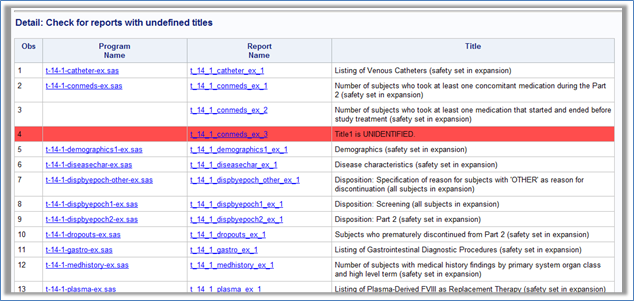
\includegraphics{image/Picture4.png}

\hypertarget{check2-check-for-missing-footnote-references}{%
\subsubsection{CHECK2: Check for missing footnote
references}\label{check2-check-for-missing-footnote-references}}

The search for possible footnote related issues includes the following:

·~~~~~~~~ Column references without a matching footnote

·~~~~~~~~ Row references without a matching footnote

·~~~~~~~~ Row header reference without a matching footnote

·~~~~~~~~ Value reference without a matching footnote

·~~~~~~~~ Footnote without the corresponding reference~

Refer to \protect\hyperlink{appendix-b}{Appendix B:~} for detail.~

\hypertarget{check3-check-for-duplicate-records-in-reports}{%
\subsubsection{CHECK3: Check for duplicate records in
reports}\label{check3-check-for-duplicate-records-in-reports}}

This is about identifying duplicate rows in the reports.

Refer to \protect\hyperlink{appendix-c}{APPENDIX C:} for detail.

\hypertarget{check4-check-report-creation-dates}{%
\subsubsection{CHECK4: Check report creation
dates}\label{check4-check-report-creation-dates}}

If the gap between report creation date and that of the most recent
report is greater than \&TIMING\_WINDOW seconds, the report is flagged.

Sample report:

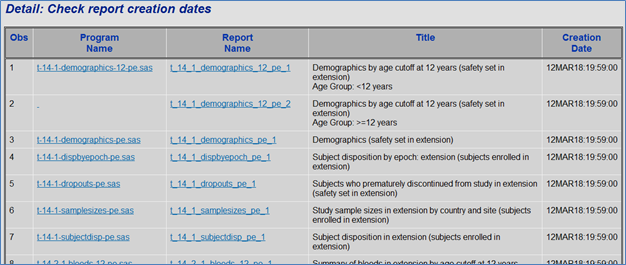
\includegraphics{image/Picture5.png}

\hypertarget{check5}{%
\subsubsection{CHECK5:}\label{check5}}

\hypertarget{compare-program-file-names-against-name-parameter-in-iniprog-call}{%
\paragraph{Compare program file names against NAME parameter in
\%iniprog
call}\label{compare-program-file-names-against-name-parameter-in-iniprog-call}}

\textbf{The report is flagged if NAME parameter in \%iniprog call does
not match the file name.}

Sample report:\\
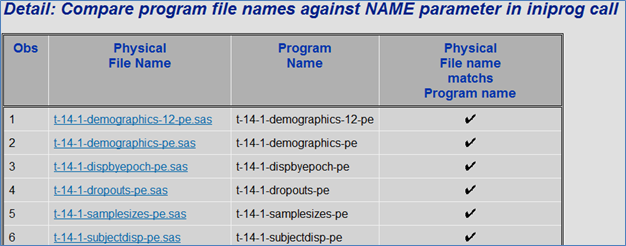
\includegraphics{image/Picture6.png}

\hypertarget{check6-check-for-empty-reports}{%
\subsubsection{CHECK6: Check for empty
reports}\label{check6-check-for-empty-reports}}

All reports that contain no data are flagged.

Sample report:

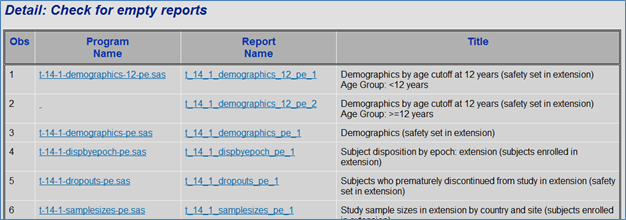
\includegraphics{image/Picture7.png}

\hypertarget{check7-check-for-missing-iniprog-andor-endprog-calls}{%
\subsubsection{CHECK7: Check for missing \%iniprog and/or \%endprog
calls}\label{check7-check-for-missing-iniprog-andor-endprog-calls}}

SAS programs are scanned for presence of \%iniprog and \%endprog calls.
Reports that do not contain either of them are flagged.

For Example:

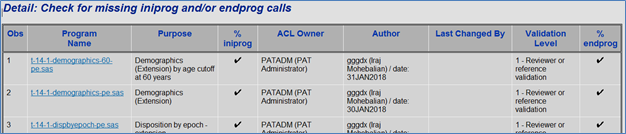
\includegraphics{image/Picture8.png}

Note: ACL Owner column indicates the Unix ownership of the file. It is
the output of the ``ls --la'' command.

Columns Purpose, Author, Last Changed By, and Validation Level are the
text retrieved from the program's header.~~

\hypertarget{check8}{%
\subsubsection{CHECK8:}\label{check8}}

\hypertarget{check-sas-log-files}{%
\subsubsection{Check SAS log files}\label{check-sas-log-files}}

SAS log files are scanned for presence of ERRORs, WARNINGs and critical
NOTEs. Reports are flagged if any such lines are detected.

Sample Report:

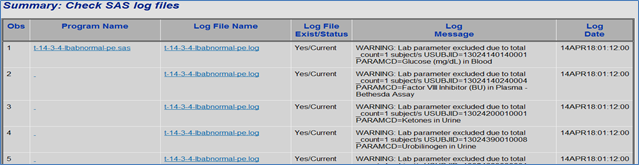
\includegraphics{image/Picture9.png}

\hypertarget{check9}{%
\subsubsection{CHECK9:}\label{check9}}

\hypertarget{check-ae-reports-for-discrepancies}{%
\subsubsection{Check AE reports for
discrepancies}\label{check-ae-reports-for-discrepancies}}

Check numbers among AE Summary, Overall and Listing reports.

AE reports are grouped to the following categories:~~

\ul{\textbf{Population Set}}: safety analysis set, full analysis set,
intent-to-treat, per-protocol,\ldots.

\ul{\textbf{Timing Method:}}\_all\_, Treatment Emergent, Cutoff, After,
Before, Between, Phase, Pre/Post treatment, Page Title

\ul{\textbf{Scope:}}~ Any AE, SAE, Severe, Related, SAE,
Discontinuation, non-Serious

\ul{\textbf{Dictionary:}}MedDRA, CTCAE,~ MedDRA/CTCAE, not specific is
default to MedDRA

Reported numbers between each group has to match.

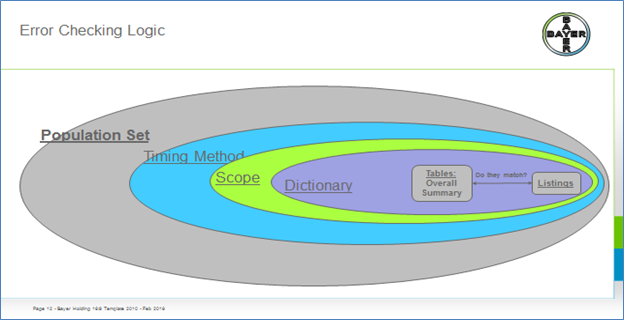
\includegraphics{image/Picture10.png}

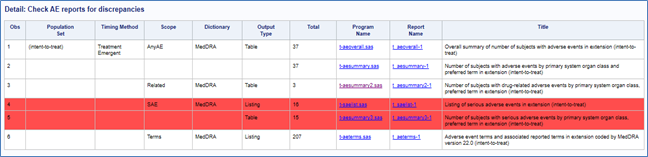
\includegraphics{image/Picture11.png}

\hypertarget{check10}{%
\subsubsection{CHECK10:}\label{check10}}

\hypertarget{check-big-n-within-each-population-group}{%
\subsubsection{Check Big N within each population
group}\label{check-big-n-within-each-population-group}}

Check reports for discrepancies in reporting Big N for various
populations.~ Reports that their Big N do not match within a population
are flagged.

Sample HTML detail report using SAS 9.4:

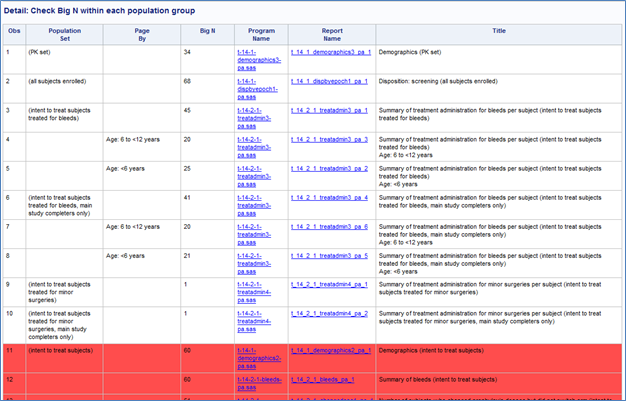
\includegraphics[width=5.84375in,height=\textheight]{image/Picture12.png}

\hypertarget{check11}{%
\subsubsection{CHECK11:}\label{check11}}

\hypertarget{check-for-hardcoded-libnames-and-formats}{%
\subsubsection{Check for hardcoded libnames and
formats}\label{check-for-hardcoded-libnames-and-formats}}

Check for hardcoded libnames and formats. SAS programs are scanned for
presence of LIBNAME and PROC FORMAT words. Reports that contain either
of them are flagged.

Sample HTML detail report using SAS 9.4:

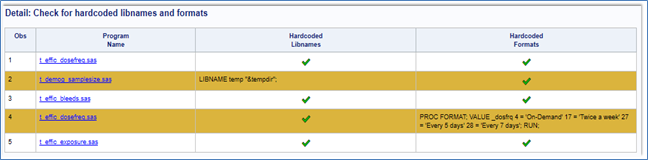
\includegraphics{image/Picture13.png}

\hypertarget{check12}{%
\subsubsection{CHECK12:}\label{check12}}

\hypertarget{check-for-reports-with-invalid-values}{%
\subsubsection{Check for reports with invalid
values}\label{check-for-reports-with-invalid-values}}

Check for reports with invalid values.

~For example:

~~~~~~~~~~~ 1. Check for UNCODED! fields.

~~~~~~~~~~~ 2. in case Taiwan is used in a Table, the following two
checks are applied:\\
\hspace*{0.333em}\hspace*{0.333em}\hspace*{0.333em}\hspace*{0.333em}\hspace*{0.333em}\hspace*{0.333em}\hspace*{0.333em}\hspace*{0.333em}\hspace*{0.333em}\hspace*{0.333em}\hspace*{0.333em}
1.) If Country is used, it should always be ``Country / Region''. This
is also required for all titles ~~~~~ and footnotes.\\
\hspace*{0.333em}\hspace*{0.333em}\hspace*{0.333em}\hspace*{0.333em}\hspace*{0.333em}\hspace*{0.333em}\hspace*{0.333em}\hspace*{0.333em}\hspace*{0.333em}\hspace*{0.333em}\hspace*{0.333em}
2.) In no case the term ``Province of China'' should be used in
combination with Taiwan\\
\hspace*{0.333em}\hspace*{0.333em}\hspace*{0.333em}\hspace*{0.333em}\hspace*{0.333em}\hspace*{0.333em}\hspace*{0.333em}\hspace*{0.333em}\hspace*{0.333em}\hspace*{0.333em}\hspace*{0.333em}
Both checks are required to ensure we apply to all requirements for
submissions in China and Taiwan.

~~~~~~~~~~~ 3. Check for reports with invalid value of ``\&''.

Sample HTML summary report using SAS 9.4:

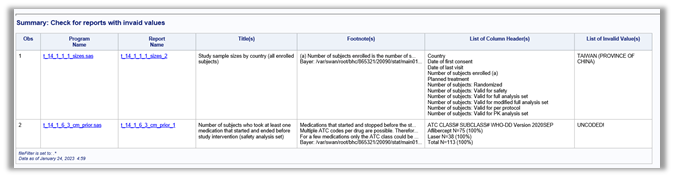
\includegraphics{image/Picture14.png}

\hypertarget{checkx-run-study-specific-checks}{%
\subsubsection{CHECKX: Run study specific
checks}\label{checkx-run-study-specific-checks}}

The default for this parameter is NO. When it is changed to YES, macro
\%CRV\_CheckX0 is executed if it is defined. The macro is expected to
contain study-specific checks.

\hypertarget{report_type}{%
\subsubsection{REPORT\_TYPE}\label{report_type}}

This parameter determines whether the output is stored in HTML or RTF
formats, or both if it is set to ALL (default).

\hypertarget{filefilter}{%
\subsubsection{FILEFILTER}\label{filefilter}}

This parameter defines a regular expression to subset specific reports.
The default is ``.*'', which selects every existing report.

\hypertarget{colors}{%
\subsubsection{COLORS}\label{colors}}

This parameter defines the colors used for flagged records in the
reports. The default is set to Orange\textbar Yellow.

1\textsuperscript{st} color in the list used for the failed checks.
2\textsuperscript{nd} color in the list is used for the TBD checks.~

\hypertarget{keyword}{%
\subsubsection{KEYWORD}\label{keyword}}

Optional text string to identify missing titles. A report is considered
having an undefined title if TITLE1 is missing or contains \&KEYWORD.
The default for the parameter KEYWORD is ``UNIDENTIFIED''.

\hypertarget{firstobs}{%
\subsubsection{FIRSTOBS}\label{firstobs}}

It is used to limit the number of reports to check.~ Because of memory
issue, we may need to limit the number of reports to check. It specifies
the first observation to process.

\hypertarget{obs}{%
\subsubsection{OBS}\label{obs}}

It specifies the last observation to process. When FIRSTOBS is not also
used, this corresponds to the number of observations that will be read.
The default value is set to Max.

Following is an example of selecting only the 5000 reports:

\emph{\%crv\_check(obs=5000)}

\hypertarget{search_column_header}{%
\subsubsection{SEARCH\_COLUMN\_HEADER}\label{search_column_header}}

This parameter defines a column header to search. The default is
``Total'', which select columns with the header of ``Total''.

\hypertarget{timing_window}{%
\subsubsection{TIMING\_WINDOW}\label{timing_window}}

This parameter sets maximal time span, in seconds, allowed between
individual reports. The default value is 21600, which is an equivalent
of 6 hours.

\hypertarget{help}{%
\subsubsection{HELP}\label{help}}

The default for this parameter is NO. When it is changed to YES, help
text is printed to the SAS log.

\hypertarget{verbose}{%
\subsubsection{VERBOSE}\label{verbose}}

The default for this parameter is NO. When it is changed to YES, general
messages (including starting and finishing information) are printed to
the SAS log. With the default setting, only ERROR and WARNING messages
are printed.

\hypertarget{checks-and-error-handling}{%
\subsection{Checks and Error Handling}\label{checks-and-error-handling}}

The following checks and error handlings are performed.

\begin{longtable}[]{@{}
  >{\raggedright\arraybackslash}p{(\columnwidth - 6\tabcolsep) * \real{0.1377}}
  >{\raggedright\arraybackslash}p{(\columnwidth - 6\tabcolsep) * \real{0.1159}}
  >{\raggedright\arraybackslash}p{(\columnwidth - 6\tabcolsep) * \real{0.5362}}
  >{\raggedright\arraybackslash}p{(\columnwidth - 6\tabcolsep) * \real{0.2101}}@{}}
\toprule\noalign{}
\endhead
\bottomrule\noalign{}
\endlastfoot
& & & \\
\textbf{Type of check} & \textbf{Object} & \textbf{Descriptions} &
\textbf{Message / Reaction} \\
& & & \\
FORMAL & LIB & Must be a valid existing library & Abort with an error
message \\
& & & \\
FORMAL & METADATA & Must be existing dataset(s) (also in combination
with INLIB if provided) & Abort with an error message \\
& & & \\
FORMAL & LIB METADATA & LIB and METADATA must not be both missing &
Abort with an error message \\
& & & \\
FORMAL & REPORT\_TYPE & Must use HTM, RTF or ALL & Abort with an error
message \\
& & & \\
FORMAL & CHECK1-CHECK12 & Must either be N(O) or Y(ES) & Abort with an
error message \\
& & & \\
FORMAL & CHECKX & Must either be N(O) or Y(ES) & Abort with an error
message \\
& & & \\
FORMAL & FIRSTOBS & Must be a valid integer number. Cannot be empty. &
Abort with an error message \\
& & & \\
FORMAL & OBS & Must be a valid integer number. Cannot be empty. & Abort
with an error message \\
& & & \\
FORMAL & TIMING\_FLAG & Must be a NUMERIC & Abort with an error
message \\
& & & \\
FORMAL & HELP & Must either be N(O) or Y(ES) & Abort with an error
message \\
& & & \\
FORMAL & VERBOSE & Must either be N(O) or Y(ES) & Abort with an error
message \\
& & & \\
\end{longtable}

\hypertarget{processing-steps}{%
\subsection{Processing Steps}\label{processing-steps}}

CRV\_check macro relies on the datalist metadata to identify
discrepancies in the tables and reports.~ To create ~datalist metadata
for a study, add the following lines to your run\_all.sas program:

\%initsystems(initstudy=5)

\%initstudy(\ldots\ldots.)

\%startMostoMetadata()

\hypertarget{output-generation}{%
\subsection{Output Generation}\label{output-generation}}

Based on the REPORT\_TYPE parameter, CRV\_Check macro generates an .HTM
and/or a .RTF file(s) that includes the results from all the checks.

Example:

Clicking of the ``Obs'' number, detail report of the selected check will
be displayed. Clicking on the ``Status'' column, summary report of the
selected check will be displayed. ~

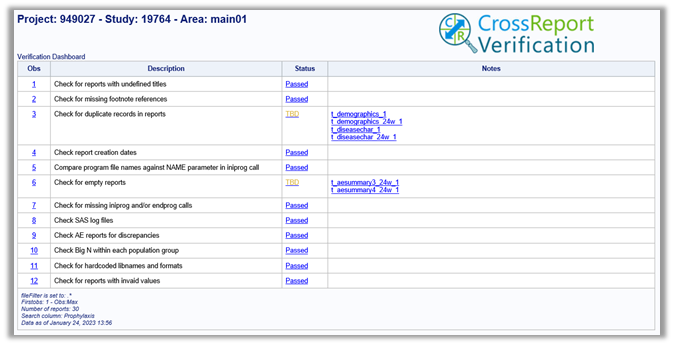
\includegraphics{image/Picture15.png}

To generate the above report, run the \%crv\_check macro at the end of
your run\_all.sas program.

Or, you may also want to create a separate run\_crv file to generate the
report.

For example:

\%initsystems(initstudy=5, spro=3, crv=2)

\%initstudy()

\%crv\_check;

\hypertarget{status}{%
\subsection{Status}\label{status}}

Status field has the following options: Passed, Failed and TBD
(To-Be-Determined).

•~~~~~~ \textbf{Passed:} I know the values are correct.

•~~~~~~ \textbf{Failed}: I know the values are incorrect.

•~~~~~~ \textbf{TBD}: I don't know if the values are correct.

For some checks, by checking, I know that the values are correct or not.
Passed or Failed.~ Checks like looking for missing titles. Titles are
there or not? Yes or No

Some checks like check\#3, find duplicate records, it totally depends on
the report.~ You can easily find duplicate records in the demography
report.~ But in the death report, you don't want to find duplicates.

TBD is for those cases where the program cannot figure whether something
is correct or not, so they need to be checked visually.

Following is a list of valid status values for each check:

Default colors associated with status values are:

Within the CRV reports, there are default colors associated with these
values: Yellow for ``TBD'', Orange for ``Failed'', default SAS
background color for ``Passed''. When running CRV in SAS 9.2, default
background color is ``Gray''. Running it with SAS 9.4, default
background color is ``White''.

You can change these default colors with the use of CRV macro parameter.

\hypertarget{constraints}{%
\subsection{1.6~~~~~~~~ Constraints}\label{constraints}}

If your study has multiple runall programs, and you want to run them all
at the same time, you need to specify a unique metadat parameter for the
\%startMostoMetadata macro.

For Example:~~

\%startmostometadata(metadat=tlfmeta.META\_Section14);

\%startmostometadata(metadat=tlfmeta.META\_Section16);

\hypertarget{documentfinish}{%
\section{2.~~~ \%DocumentFinish}\label{documentfinish}}

Following are the steps for storing the crv\_check findings to a MS-Word
document:

1.~~~~ Copy the
\href{file://by-sas2p.bayer-ag.com/patdb/std_sg/stat/systems/crv/doc/crv2/template_crv_check.doc}{\textbackslash\textbackslash by-sas2p.bayer-ag.com\textbackslash patdb\textbackslash std\_sg\textbackslash stat\textbackslash systems\textbackslash crv\textbackslash doc\textbackslash crv2\textbackslash template\_crv\_check.doc}
file to your study .pgm directory.

2.~~~~ Update the template\_crv.doc header information.

3.~~~~ Add the following line to your runall program:

\%DocumentFinish(template=template\_CRV\_check.doc, tmpldir=\&prgdir,
\_outdir=\&outdir, ResultPrefix= )

Sample CRV\_Check.doc file:

\hypertarget{appendix-a-overall-report-structure}{%
\section{3.Appendix A: overall report
structure}\label{appendix-a-overall-report-structure}}

Following is the overall structure of the html file generated by the
CRV\_CHECK:

\begin{longtable}[]{@{}
  >{\raggedright\arraybackslash}p{(\columnwidth - 4\tabcolsep) * \real{0.0385}}
  >{\raggedright\arraybackslash}p{(\columnwidth - 4\tabcolsep) * \real{0.9135}}
  >{\raggedright\arraybackslash}p{(\columnwidth - 4\tabcolsep) * \real{0.0385}}@{}}
\toprule\noalign{}
\endhead
\bottomrule\noalign{}
\endlastfoot
& & \\
& \begin{minipage}[t]{\linewidth}\raggedright
\begin{longtable}[]{@{}
  >{\raggedright\arraybackslash}p{(\columnwidth - 4\tabcolsep) * \real{0.0435}}
  >{\raggedright\arraybackslash}p{(\columnwidth - 4\tabcolsep) * \real{0.9022}}
  >{\raggedright\arraybackslash}p{(\columnwidth - 4\tabcolsep) * \real{0.0435}}@{}}
\toprule\noalign{}
\endhead
\bottomrule\noalign{}
\endlastfoot
& & \\
& Table of C

\includegraphics{file:///C:/Users/EMVSX/AppData/Local/Temp/msohtmlclip1/01/clip_image034.png}
& \\
& & \\
\end{longtable}
\end{minipage} & \\
& & \\
\end{longtable}

\begin{longtable}[]{@{}
  >{\raggedright\arraybackslash}p{(\columnwidth - 4\tabcolsep) * \real{0.0435}}
  >{\raggedright\arraybackslash}p{(\columnwidth - 4\tabcolsep) * \real{0.9022}}
  >{\raggedright\arraybackslash}p{(\columnwidth - 4\tabcolsep) * \real{0.0435}}@{}}
\toprule\noalign{}
\endhead
\bottomrule\noalign{}
\endlastfoot
& & \\
& Table of C

\includegraphics{file:///C:/Users/EMVSX/AppData/Local/Temp/msohtmlclip1/01/clip_image034.png}
& \\
& & \\
\end{longtable}

~~~~~~~~~~~~~~~~~~~~~~~~~~~~~~~~~~~~~~~~~~~~~~~~~~~~~~~~~~~~~~~~~~~~~~~~~~~~~~~~~~~~~~~~~~~~~~~~~~~~~~~~~~~~~~~~~~~~~~~~~~~~~~~~~~~~~~~~~~~~~~~~~~~~~~~~
~~~~~~~~~~~~~~~~~~~~~~~~~~~~~~~~~~~~~~~~~~~~~~~~~~~~~~~~~~~~~~~~~~~~~~~~~~~~~~~~~~~~~~~~~~~~~~~~~~~~~~~~~~~~~~~~~~~~~~~~~~~~~~~~~~~~~~~~~~~~~~~~~~~~~~~~~~~~~~~~~~~~~~~
~~~~~~~~~~~

\hypertarget{appendix-b}{%
\section{Appendix B:~}\label{appendix-b}}

\hypertarget{examples-of-footnote-reference-issues}{%
\subsubsection{Examples of footnote reference
issues}\label{examples-of-footnote-reference-issues}}

Following are examples of various missing footnote references: ~

Column reference missing footnote:

Row reference missing footnote

Footnote without any reference

Summary check report for the above report:

\hypertarget{appendix-c}{%
\section{APPENDIX C:}\label{appendix-c}}

\hypertarget{example-of-a-report-with-duplicate-records}{%
\section{Example of a report with duplicate
records}\label{example-of-a-report-with-duplicate-records}}

Following is a sample summary report that shows reports with a number of
duplicate records.

For example, in the first row, it shows we have three duplicate AE
records.

Clicking on the number 3 in the duplicate records column will display
the duplicate records.~~

Example of checking for duplicate records in a report:~

By clicking on the report name on the last line, it will take you to the
report.

Following is the snapshot of the actual report, with its duplicate
records.

When running a check against a study that includes the above report,
this discrepancy will be identified.~~

First row in the following summary report shows there are three
duplicate AE records.

Clicking on the number ``3'' in the duplicate records column will
display the three duplicate records.~~

Following report indicates three separate duplicate records in the AE
listing.~

Clicking on the report name on the last line will display the actual
report.



\end{document}
